\begin{problem}%
{Кампус}%
{\textsl{стандартный ввод}}%
{\textsl{стандартный вывод}}%
{1 секунда}%
{256 мегабайт}{}

Новое здание кампуса Университета Байтбурга имеет n этажей, пронумерованных снизу вверх от $1$ до $n$. Комнаты студентов расположены в нескольких подъездах.\\

В каждом подъезде на этажах, номер которых кратен числу $k$, расположено по $x$ комнат, а на остальных этажах расположено по $y$ комнат.\\

Комнаты внутри каждого подъезда пронумерованы последовательными
натуральными числами. Номера комнат на первом этаже имеют наименьшие значения в этом подъезде, затем следуют номера комнат на втором этаже, и так далее. Комнаты в первом подъезде пронумерованы, начиная с 1, в каждом следующем подъезде нумерация комнат начинается с числа, следующего после максимального номера комнаты в предыдущем
подъезде.\\

На рис. 1 показаны номера комнат в здании с $n = 7$ этажами, 3 подъездами, и
параметрами $k = 3$, $x = 2$, $y = 3$.

\begin{center}
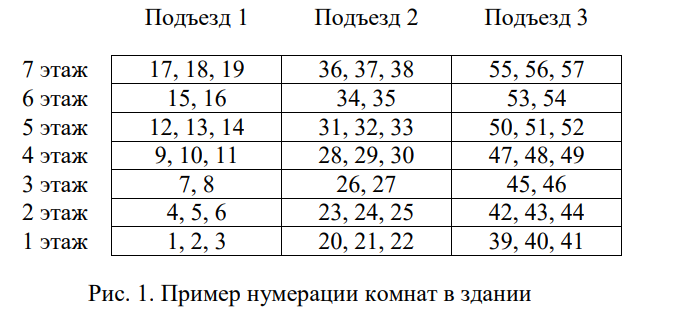
\includegraphics[scale=0.5]{images/5.png}
\end{center}

Для организации расселения студентов администрация кампуса должна по номеру комнаты оперативно определять этаж, на котором она находится.\\

Требуется написать программу, которая по заданным числам $n$, $k$, $x$ и $y$, а также по номерам комнат, определяет для каждой комнаты, на каком этаже она находится.

\InputFile

Первая строка входного файла содержит натуральные числа $n$, $k$, $x$ и $y$ ($1 \le n \le 10^9$, $1 \le k \le n$, $1 \le x, y \le 10^9$). Соседние числа разделены ровно одним пробелом.\\

Вторая строка входного файла содержит натуральное число $q$ — количество номеров комнат, для которых требуется определить этаж ($1 \le q \le 1000$).\\

Третья строка содержит $q$ целых чисел $a_1$, $a_2$, \dots, $a_q$ — номера комнат ($1 \le a_i \le 10^{18}$). Можно считать, что в здании так много подъездов, что все комнаты с заданными номерами
существуют.

\OutputFile

Требуется вывести $q$ чисел, по одному на строке. Для каждого номера комнаты во входном файле требуется вывести номер этажа, на котором она находится.

\Examples

\begin{example}
\exmp{
7 3 2 3
4
1 19 20 50
}{%
1
7
1
5
}%
\end{example}
\end{problem}
